\documentclass[12pt,letterpaper]{article}
\usepackage{graphicx}
\usepackage{scrextend}
\usepackage{vmargin}
\usepackage{graphicx}
\usepackage{multirow}
\usepackage[utf8]{inputenc}
\usepackage[spanish]{babel}
\usepackage{multicol}
\usepackage{enumerate}
\usepackage{float}
\usepackage{amsmath, amsthm, amssymb, amsfonts}
\usepackage[usenames]{color}
\usepackage[breaklinks=true,hidelinks]{hyperref}
\parindent=0mm
\pagestyle{empty}
\definecolor{miorange}{rgb}{0.91, 0.43, 0.0}
\begin{document}
\setmargins{2.5cm}      
{1.5cm}                     
{2cm}  
{24cm}                    
{10pt}                          
{1cm}                          
{0pt}                             
{2cm}
\begin{titlepage}
\begin{center}

\includegraphics[scale=0.40]{../../../Logos/uanl.png} 
\hspace{2.5cm}

\includegraphics[scale=0.40]{../../../Logos/fcfm.png}
\end{center}
\vspace{2cm}
\begin{center}
\textbf{
UNIVERSIDAD AUTÓNOMA DE NUEVO LEÓN\\
FACULTAD DE CIENCIAS
FÍSICO MATEMÁTICAS}\\
\vspace*{2cm}
\begin{large}
\vspace{1cm}
\large{\textbf{Aplicaciones de la Mecánica Cuántica}}\\
\textbf{Radiación de fondo de microondas}\\
Carlos Luna Criado\\
\end{large}
\vspace{3.5cm}
\begin{minipage}{0.6\linewidth}
\vspace{0.5cm}
\changefontsizes{14pt}
Nombre:\\
Giovanni Gamaliel López Padilla\\
\end{minipage}
\begin{minipage}{0.2\linewidth}
\changefontsizes{14pt}
Matricula:\\
1837522
\end{minipage}
\end{center}
\vspace{4cm}
\begin{flushright}
\today
\end{flushright}
\end{titlepage}
\begin{multicols}{2}
\section*{Introducción}
\begin{figure}[H]
    \hspace{-0.5cm}
    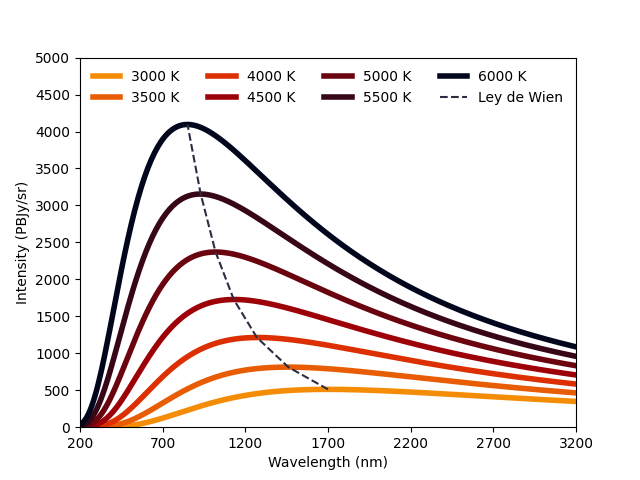
\includegraphics[scale=0.5]{../Graphics/black_body.png}
    \caption{Ecuación de cuerpo negro para diferentes temperaturas.}
    \label{black_body}
\end{figure}
\section*{Metodología}
\begin{equation}
S(\nu,T)= \frac{2h\nu^3}{c^2} \frac{1}{e^{h\nu/kT}-1}
\label{body equation}
\end{equation}
\begin{figure}[H]
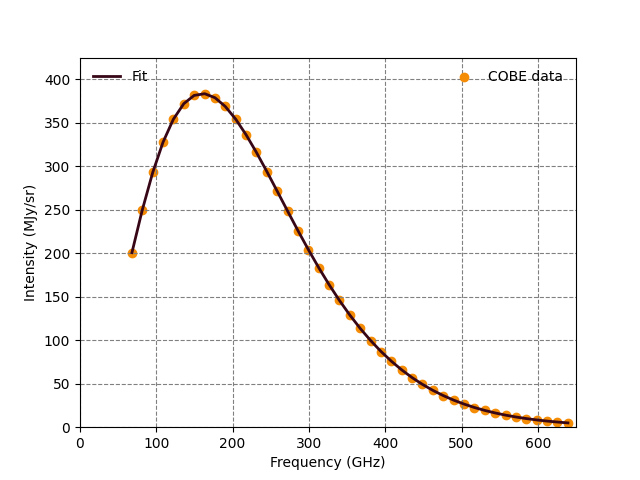
\includegraphics[scale=0.45]{../Graphics/fit.png}
\caption{Fit de los datos proporcionados por el satelite FIRAS de la misión COBEA}
\end{figure}
\section*{Resultados}
\begin{equation*}
    T=2.72502K
\end{equation*}
\begin{equation*}
    RD_i = \frac{|S_i(\nu,T)-COBE_i|}{COBE_i}*100\%
\end{equation*}
\begin{equation*}
    \langle RD \rangle = \sum\limits_{i=1}^N \frac{RD_i}{N} = 0.3205\%
\end{equation*}
\begin{equation*}
    R^2=0.99999972482939
    \label{coef_deter}
\end{equation*}
\section*{Conclusiones}
\bibliographystyle{plain}
\bibliography{Main}
\nocite{*}
\section*{Código}
\href{https://github.com/giovannilopez9808/Notas_Agosto_2020/blob/master/AMC/Reto1/fit.py}{Github - black_body.py}
\end{multicols}
\end{document}